\documentclass{article}

\usepackage{url}
\usepackage{tikz}
\usepackage{float}
\usepackage{amsmath}
\usepackage{enumitem}

\usetikzlibrary{matrix, shapes, snakes, arrows}
\tikzset{>=triangle 45}

\title{CS 612: Assignment 1\\Spring 2013}

\author{Dustin Ingram}

\date{\today}

\begin{document}

\maketitle

\section*{Written}

\begin{enumerate}[label=(\alph*)]

\item{} % a

The first issue to solve is the configuration of the predators. Each predator
must be in one of the four positions around a prey, and they cannot duplicate
the position with another predator.

Without communication, the predators would need a way to determine which
predator will take which position. Since every predator shares the same
worldview, I would propose a strategy that would guarantee that each predator
can individually make the same decision about the optimal position for every
predator in the world, and thus arrive at the same configuration, and thus
coordinate their positions.

The resulting algorithm might be as follows: for every position around the prey,
in the order N, S, E, W, find the predator that is closest to that position and
``assign'' that predator to that position. Once every predator has been assigned
a position, the predator running the algorithm knows it's position, and the
result is guaranteed to be the same for all the other predators as well. The
predators can even continue to use the same positions for every subsequent prey
(i.e., one predator is always N, one is always S, etc.)

The next issue to solve is determining which prey to pursue first. Again, in
order for the predators to be able to coordinate without communication, they
must all use an algorithm which depends on the world state, and is guaranteed to
arrive at the same result.

Here, the resulting algorithm might be as follows: for every prey, every
predator calculates the average distance between that prey and every predator.
Then the predator determines to pursue the prey with the lowest average
distance.

The issue with this approach is the coordination over time. Each predator will
need to be continuously running their algorithm every time the world changes, to
ensure that their efforts are coordinated, since it might be possible for the
world to change while the predators are planning, and might result in different
strategies. This might be an inefficient strategy overall, as the closest prey
might be constantly changing, and thus the target constantly changing as well.

\item{} % b

If the predators can communicate with each other, this does not necessarily
help the effectiveness of the predators strategy.

In terms of positioning, the original strategy would work fine without
communication.

At the beginning of the simulation (or every time a prey is captured), the
predators can run their algorithm a single time and announce which prey they
plan to pursue. If a predator receives this communication and hasn't yet
finished determining which prey to pursue on their own, they can effectively
follow the lead of the other predator until that prey is captured, and thus not
need to 

There may be a large number of issues if the predators only have a range of
sight or communication, but this is likely outside the scope of this problem.

\end{enumerate}

\section*{Programming}

\begin{enumerate}

\item{} % 1

I implemented the code to simulate the termites in Python as specified. My code
consists of the following files:
\begin{itemize}
    \item \texttt{world.py} - The representation of the termites' ``world'';
    \item \texttt{termite.py} - A representation of a termite, which has
    direction and the ability to move, as well as hold and move a piece of wood;
    \item \texttt{wood.py} - A representation of a piece of wood;
    \item \texttt{display.py} - A class specific to displaying the state of the
    ``world'' in a PyGame window;
    \item \texttt{termites.py} - The main script which runs an experiment and
    can be run from the command line.
\end{itemize}

The \texttt{termites.py} script can be run from the command line as follows:

\texttt{python termites.py -e 100}

It also accepts an optional parameter to run in command-line mode only:

\texttt{python termites.py -e 100 -c}

Running an experiment returns a object containing the results. The
\texttt{termites.py} script will output this to stdout. The format of this
object is a list of tuples, with each tuple having the format:

$$ (iterations, (n_{piles}, n_{mixed-piles})) $$

where $iterations$ is the number of steps the emulation has taken, $n_{piles}$
is the number of piles at that point in the simulation, and $n_{mixed-piles}$ is
the number of piles with multiple types (for use in part 7).

Furthermore, I created a number of scripts which run the experiments and produce
the plots for their respective parts of the assignment. They are:

\begin{itemize}
    \item \texttt{part3.py}
    \item \texttt{part4.py}
    \item \texttt{part5.py}
    \item \texttt{part7.py}
\end{itemize}

They can be run to generate the plot for their respective sections as follows:

\texttt{python part3.py}

\begin{figure}[H]
\centering
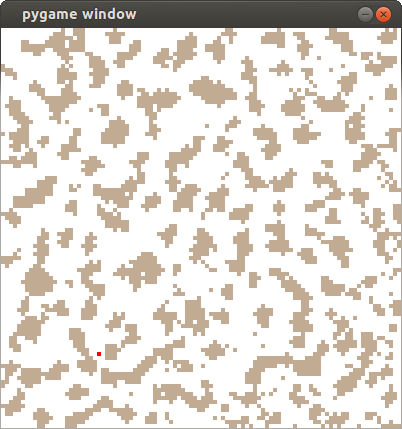
\includegraphics[width=0.65\textwidth]{figs/part_1_1.png}
\caption{A screenshot of the program with a single termite and a single wood
type after 100,000 iterations.}
\end{figure}

\begin{figure}[H]
\centering
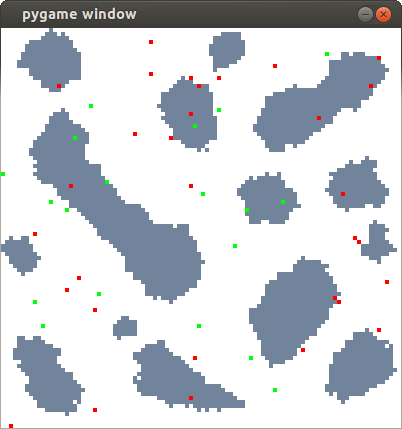
\includegraphics[width=0.65\textwidth]{figs/part_1_2.png}
\caption{A screenshot of the program with fifty termites and a single wood type
after 100,000 iterations.}
\end{figure}

The color of the wood is randomly generated. The termites are indicated as green
or red pixels, depending on whether they are currently carrying a piece of wood,
or not.

\item{} % 2

I implemented code to count the number of piles. This is the \texttt{pile\_count}
function in the \texttt{world} class. This algorithm maintains two sets of
cells:

\begin{itemize}
    \item $occupied$, a set of every cell in the grid which has a piece of wood in it;
    \item $to\_search$, a set of neighbor cells of a single original cell, all
    of whose neighbors have not necessarily been added to the set yet. 

\end{itemize}

At every iteration, it pops one cell from the $occupied$ set and onto the
$to\_search$ set, and increments the total count of piles. Then, for every cell
$c$ in the $to\_search$ set, the algorithm removes that cell from the set. For
every neighbor of $c$ which is in $occupied$, the algorithm removes that
neighbor cell from $occupied$ and adds it to $to\_search$. Once the $to\_search$
set is empty, the ``pile neighbors'' of the original cell $c$ have been
exhausted and the iteration is finished, and moves on to the next pile. Once the
$occupied$ set is empty, all occupied cells have been included in the total pile
count, and the algorithm is finished.

\item{} % 3

I created a plot to show the trend of decreasing number of chip piles as the
number of iterations increased. I considered a chip to be in a pile with another
chip if they border on the N, S, E or W sides (not diagonals) per the original
example.

\begin{figure}[H]
\centering
\label{single}
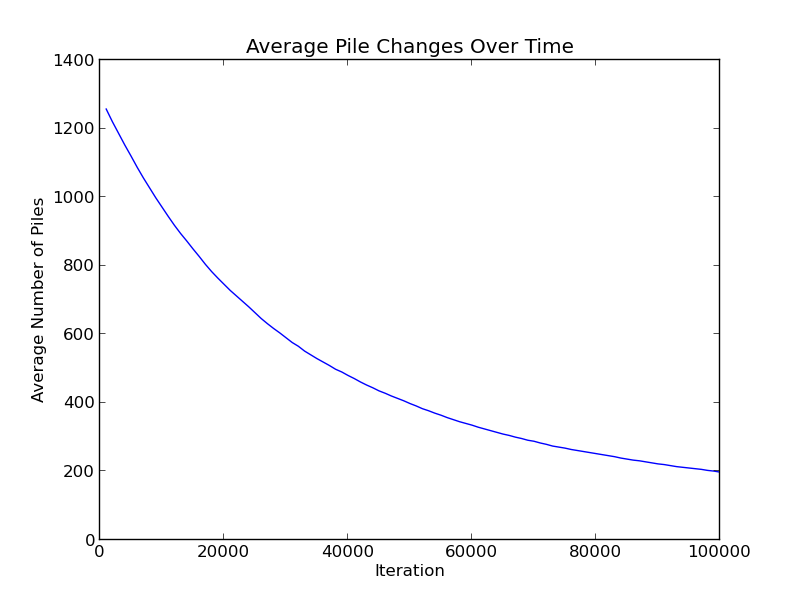
\includegraphics[width=\textwidth]{figs/part_3.png}
\caption{The average number of chip piles every 1,000 iterations over 100
experiments running for 100,000 iterations with 1 termite.}
\end{figure}

\item{} % 4

I produced 90\% confidence intervals for the preceding graph. They are extremely
tight and may be difficult to see. I have also included a detail of the same
plot. The red plot represents the upper bound, the blue plot represents the
average, and the green plot represents the lower bound.

\begin{figure}[H]
\centering
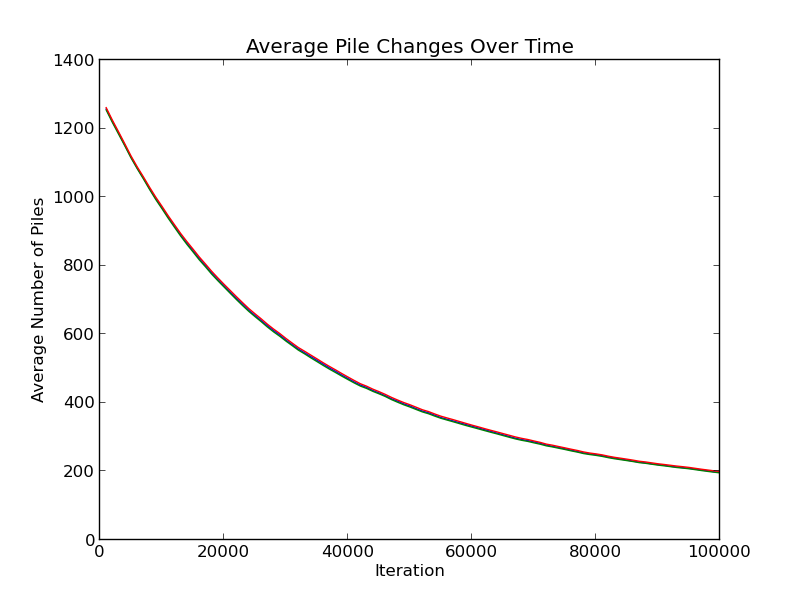
\includegraphics[width=\textwidth]{figs/part_4_1.png}
\caption{The average number of chip piles every 1,000 iterations over 100
experiments running for 100,000 iterations with 1 termite, with 90\% confidence
intervals}
\end{figure}

\begin{figure}[H]
\centering
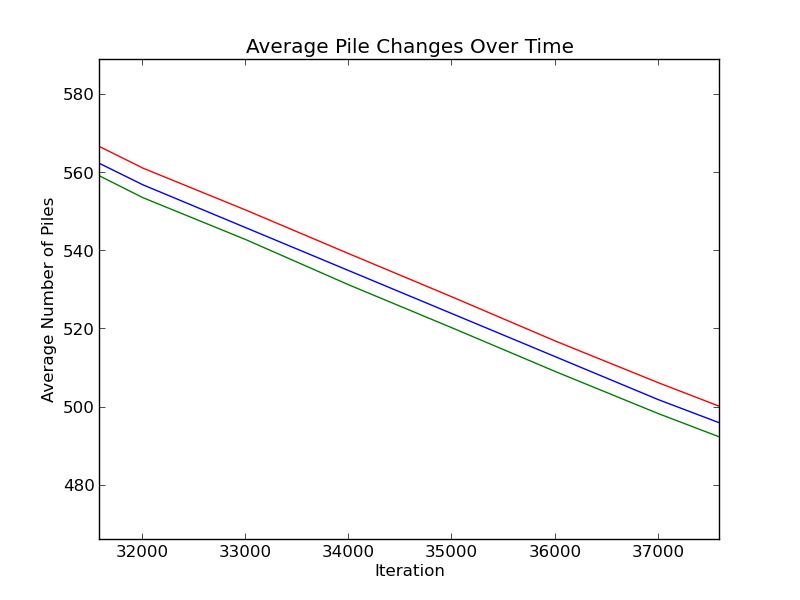
\includegraphics[width=\textwidth]{figs/part_4_2.png}
\caption{A detail of the previous figure.}
\end{figure}

\item{} % 5

I used the same parameters from part 3, but varied the number of termites from 1
to 50 termites. I also reduced the number of experiments from 100 to 10, as this
still produced a somewhat reliable average and greatly reduced the execution
time.

\begin{figure}[H]
\centering
\label{multiple}
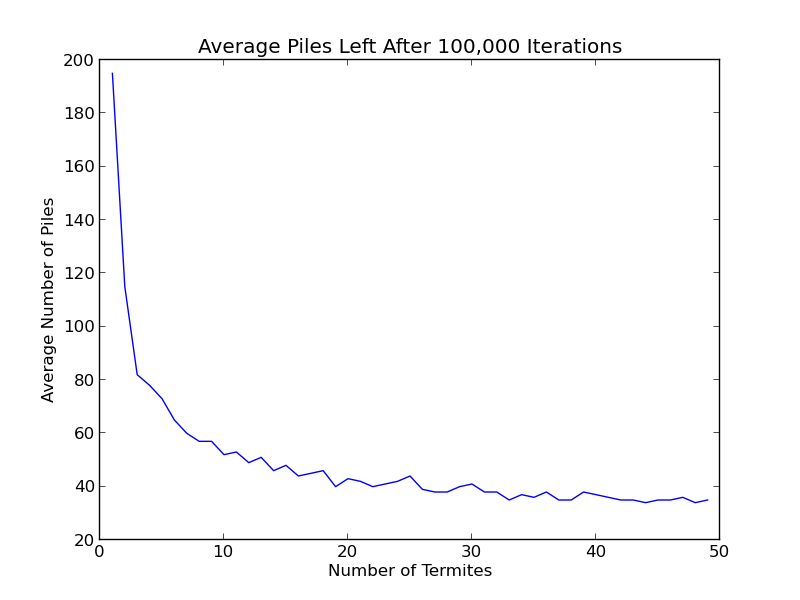
\includegraphics[width=\textwidth]{figs/part_5.png}
\caption{The average number of chip piles after 100,000 iterations over 10
experiments with a varying number of termites.}
\end{figure}

\item{} % 6

My hypothesis going into the paper was that the following basic termite behavior
would quickly converge the wood chips into piles:

\begin{itemize}
    \item \textbf{Pick up a chip if:} There is a chip in the current cell;
    \item \textbf{Drop a chip if:} The current cell neighbors a cell with a chip
    of the same type;
    \item \textbf{After dropping a chip:} Turn 180 degrees.
\end{itemize}

However, after a number of trials, it became clear that a single termite was not
producing a low enough number of piles. I then modified the termites behavior as
follows:

\begin{itemize}
    \item \textbf{Pick up a chip if:} There is a chip in the current cell, and
    it has less than five cells that border it with an identical wood type;
    \item \textbf{Drop a chip if:} The current cell neighbors a cell with at
    least two chips of the same type;
    \item \textbf{After dropping a chip:} Turn 180 degrees.
\end{itemize}

This new behavior essentially ensured that termites would not move chips which
were in the centers of the piles. It is still possible for the termites to
slowly ``eat away'' at the outside of the pile (where the neighboring chip count
is less than five), and this is how they converge pile types.

After making these changes, the simulation was able to reduce the pile count
from approx 1300 piles (the average number of piles for a $100\times 100$ grid
with density of 30\%) to less than 200 after 100,000 iterations, as is show in
Figure~\ref{single}.

My hypothesis about the effect of increasing the number of termites was that
after 100,000 iterations, the simulation with multiple termites would be able to
reduce the piles even more than the simulation with a single termite. I also
expected the simulation to converge on an amount of piles, at which point 
increasing the number of termites would have less and less effect on the number
of piles. Figure~\ref{multiple} shows this to be true, as the number of piles
converges close to 40 piles after 100,000 iterations.

To conclude, I found that my hypothesis about the behavior of a single termite
was incorrect, and I needed to give the agent slightly more intelligence before
it produced acceptable results. I found that my hypothesis about increasing the
number of termites was correct.

\item{} % 7

The simulator needed no modification to allow multiple types of wood chips. I
found that the best metric for showing how well the termites could organize
different types of wood chips into piles was the percentage of piles that had
more than one type of wood chip in them.

This metric generally decreased over time, however as the number of types of
chips grew, the constant amount of termites became worse and worse at lowering
the percentage of chips in single-type piles.

It is clear that simulations with low numbers of wood types will converge fairly
quickly (approximately after 100,000 iterations) but that for greater numbers of
types of wood, the experiment would need a large number of iterations (perhaps
several orders of magnitude more) to converge.

The behavior of the termites was not modified. The only difference is that since
there were multiple wood times, the termites would only consider the neighbors
of a cell if their wood types matched the type the termite was holding (if it
wanted to drop a piece of wood) or matched the cell in question (if it wanted to
pick up a piece of wood).

This behavior is likely the reason for the slow convergence when there is a
large number of types of wood. A termite which is less picky about the number of
matching neighbors a cell has before dropping a piece of wood would possibly
converge faster. The number of adjacent matching neighbors could even be a
function of the percentage of mixed-chip piles, so that the termites would
become pickier as the number of mixed-chip piles decreased.

\begin{figure}[H]
\centering
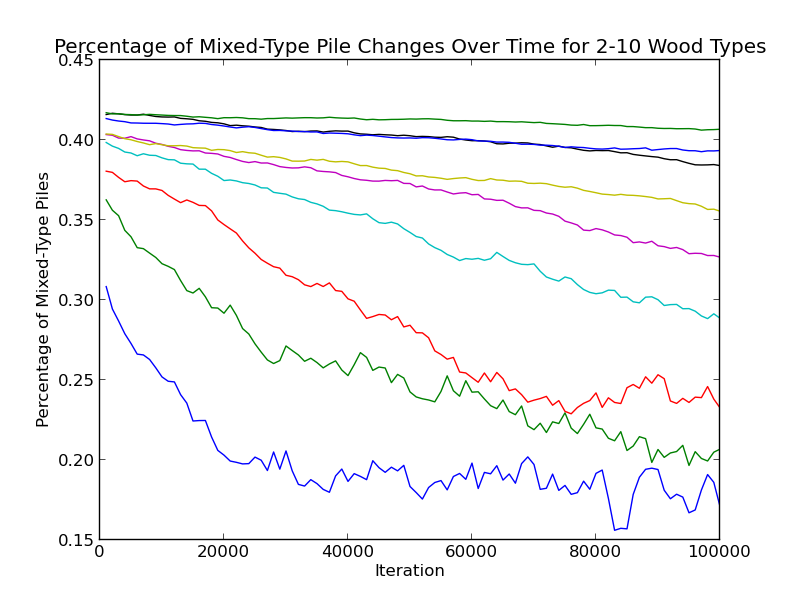
\includegraphics[width=\textwidth]{figs/part_7.png}
\caption{The average percentage of mixed-type chip piles every 1,000 iterations
over 10 experiments with 10 termites. Here, each plot represents a number of
wood types in the range $2 \ldots 10$, with the lowest (blue) plot being 2 wood
types, and the highest (bright green) being 10 wood types.}
\end{figure}

\begin{figure}[H]
\centering
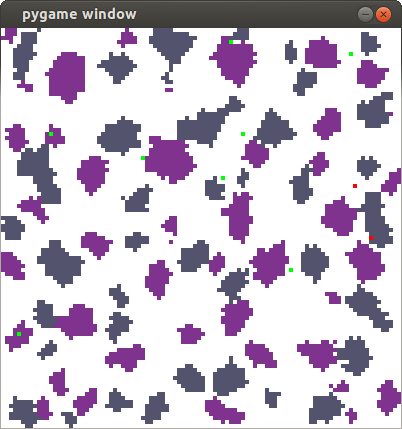
\includegraphics[width=0.65\textwidth]{figs/part_7_2.png}
\caption{Ten termites sorting two wood types after 100,000 iterations.}
\end{figure}

\begin{figure}[H]
\centering
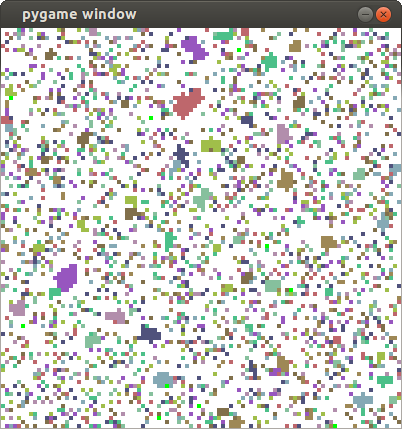
\includegraphics[width=0.65\textwidth]{figs/part_7_3.png}
\caption{Ten termites sorting ten wood types after 100,000 iterations.}
\end{figure}

\begin{figure}[H]
\centering
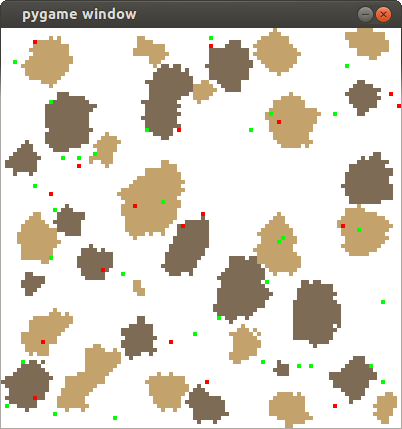
\includegraphics[width=0.65\textwidth]{figs/part_7_4.png}
\caption{Fifty termites sorting two wood types after 100,000 iterations.}
\end{figure}

\begin{figure}[H]
\centering
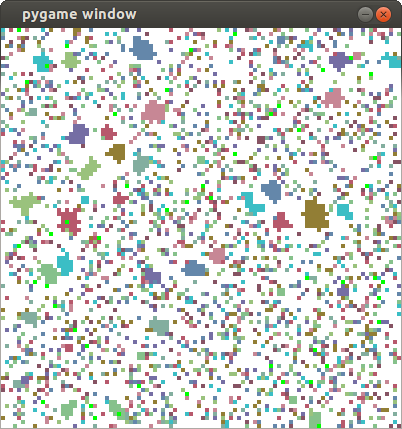
\includegraphics[width=0.65\textwidth]{figs/part_7_5.png}
\caption{Fifty termites sorting ten wood types after 100,000 iterations.}
\end{figure}

\item{} % 8

I did not do the extra-extra-credit.

\end{enumerate}

\end{document}
